\documentclass{article}[12pt]
\renewcommand{\baselinestretch}{1.5}
\setlength{\parskip}{1em}

\usepackage[parfill]{parskip}
\usepackage[affil-it]{authblk}
\usepackage[space]{grffile}

\usepackage[a4paper]{geometry}
\usepackage[latin1]{inputenc}
\usepackage[english]{babel}

\geometry{verbose}
\usepackage{float}
\usepackage{graphicx}
\usepackage{setspace}
\usepackage{caption}

\usepackage{latexsym,textcomp,longtable,tabulary}
\usepackage{booktabs,array,multirow,braket}
\usepackage{amsfonts,amsmath,amssymb,mathbbol,calc,cancel}
\usepackage{subfigure,color,blindtext,enumitem,siunitx}
\usepackage[colorinlistoftodos]{todonotes}

\usepackage{mathtools}
\usepackage{url,hyperref,etoolbox}
\numberwithin{equation}{section}
\hypersetup{colorlinks=false,pdfborder={0 0 0}}

%+figure layout options
\restylefloat{figure}
\setlist{leftmargin=*,before=\setlength{\rightmargin}{\leftmargin}}
\graphicspath{{./figures/}{docs/figures/}}

\providecommand\citet{\cite}
\providecommand\citep{\cite}
\providecommand\citealt{\cite}

\makeatletter
\makeatother

\begin{document}
\newcommand{\rates}{F_{\theta}}
\newcommand{\tangent}{T_{\theta}}
\newcommand{\steadystates}{\partial S_{\theta}}

\newcommand{\Det}{\left| \frac{\partial\rates}{\partial u} \right|}
\newcommand{\measure}{\Psi_{\theta}}

\newcommand{\predictions}{\mathcal{P}}
\newcommand{\targets}{\mathcal{D}}
\newcommand{\loss}{L}

\newcommand{\Reals}{\mathbb{R}}

\title{Inference of Bifurcations with Differentiable Continuation}
\author{Gregory Szep$^{1,2}$, Neil Dalchau$^2$ and Attila Csikasz-Nagy$^{1,3}$}
\affil{$^1$King's College London, UK, $^2$Microsoft Research Cambridge, UK, $^3$Pazmany Peter Catholic University, Budapest, Hungary}
\date{\today} \maketitle

\begin{abstract}
    In this work we propose a gradient-based semi-supervised approach for matching target bifurcations with parameterised differential equation models. The cost function contains a supervised likelihood term that is maximal when predicted bifurcations match the targets, and an unsupervised correction term that encourages bifurcations by maximising the curvature of the determinant of the Jacobian. The calculation of gradients with respect to parameters shares the same computational complexity as deflated pseudo-arclength continuation used to calculate the bifurcation diagram. We demonstrate model synthesis with minimal models which explore the space of saddle-node and pitchfork diagrams, and an applied model from synthetic biology. This work forms the basis for the inference of more complicated bifurcation diagrams which may include Andronov-Hopf points or extended to partial differential equations. 
\end{abstract}

\section{Introduction and Motivation}
\subsection{Background}
Backpropagation through differential equation solves has been a breakthrough over the past couple of years \cite{Chen2018NeuralEquations,Rackauckas2019DiffEqFlux.jl-AEquations} that enabled scalable parameter inference for differential equations. Optimisation targets, however, have mostly been expressed in the spatio-temporal domain. Acquisition of such data can be costly and can often contain over-constraining information generated by processing steps or the measurement device rather than the state variables that underpin the observed mechanism. In microscopy, for example, data is often reported in arbitrary fluoresce units allowing the observer to shift and scale data arbitrarily. Furthermore, such data may also not contain sufficient information about dynamical transients in order to identify kinetic parameters. The emerging picture suggests that identification of the qualitative dynamics -- the bifurcation diagram -- should precede any attempt at inferring kinetic parameters \cite{Stumpf2019ParameterBifurcations}.

In this work we propose a gradient-based semi-supervised approach that focuses on fitting qualitative dynamics, defined by state space structures, rather than kinetics. We find that calculating the gradients, which inform the optimisation of parameters, shares the same computational complexity as the algorithm used to calculate the bifurcation diagram. We use a predictor-corrector method called deflated pseudo-arclength continuation \cite{Farrell2016TheDiagrams,Veltz2019PseudoArcLengthContinuation.jl}. For partial differential equations, the computational complexity of calculating a single bifurcation diagram is not bounded since superpositions of localised solutions may give rise to uncountably many branches \cite{Avitabile2010ToEquation}. The complexity of computing a single branch, however, is bounded by the complexities of the chosen eigenvalue solver and corrector, and further decreased by adaptive stepping procedures \cite{Aruliah2016AlgorithmContinuation}.

We find that the cost function landscape contains basins that not only allow us to synthesise models with a desired bifurcation structure but also allow us to organise models in terms of topological and geometric equivalence. We discuss the relevance of this in model selection.

\subsection{Similar and Related Works}

\begin{itemize}
    \item smooth and match estimator methods \cite{Ranciati2017BayesianParameters}
    \item bifurcation inference using Mixed Integer Nonlinear Programming optimization strategy \cite{Otero-Muras2018Optimization-basedModels}
\end{itemize}
\clearpage

\section{Methodology}

\subsection{Problem Statement}
Suppose we parameterise a set of differential equations for states $u\in\Reals^N$ with a function $\rates$ in an unknown parameter space $\theta\in\Reals^M$. We would like these differential equations to obey a set of target bifurcations $\targets:=\{p_1\dots p_K\}$ along a known bifurcation parameter $p\in\Reals$. The following sections outline how a gradient descent algorithm could encourage predicted bifurcations $\predictions(\theta)$ coming from parameterised differential equations to match specified targets $\targets$. This would allow us to design differential equations using high-level qualitative constraints and sample qualitatively equivalent models in regions of optimal $\theta$. Let the differential equations be defined as
\begin{align}
	\partial_t u=\rates(z)
	\qquad\mathrm{where}\quad z:=(u,p)\quad
	\rates : \Reals^{N+1}\rightarrow\Reals^N
	\label{eq:model}
\end{align}

First we view the steady states of this problem in terms of implicit space curves \cite{Goldman2005CurvatureSurfaces} in an augmented state space $z\in\Reals^{N+1}$ which combines the state $u$ and bifurcation parameter $p$. We then realise that the curvature of the Jacobian determinant $\Det(z):=|\partial\rates/\partial u|$ is maximised when bifurcations appear in the observed region of $z$. Luckily the curvature can be evaluated analytically \cite{Goldman2005CurvatureSurfaces}. The steady state regions of $z$ are computed using a parameter continuation method \cite{Veltz2019PseudoArcLengthContinuation.jl,Farrell2016TheDiagrams}. Finally a differentiable semi-supervised cost function $\loss(\theta|\targets)$ is proposed that would allow gradient descent algorithms to efficiently encourage bifurcations and match their locations to targets $\targets$.

For clarity, we guide the reader through the methods with the following minimal models that explore the space of saddle-nodes $\rates(z) = p + \theta_{1}u+\theta_{2}u^3$ and pitchforks $\rates(z) = \theta_{1} + p u+\theta_{2}u^3$. These minimal models are shown with targets $\targets$ in Figure \ref{fig:saddle-node} and Figure \ref{fig:pitchfork} respectively. These figures show that the curvature of the determinant $\Det(z)$ increases in the vicinity of bifurcations and crosses zero at the bifurcations. This gives us our first hint of what should be optimised to encourage bifurcations. Success on these minimal models demonstrates the proof of concept, and success in practice is demonstrated on a four component genetic toggle switch model taken from synthetic biology.
\begin{figure}[H]
\centering{}
\captionsetup{justification=centering}
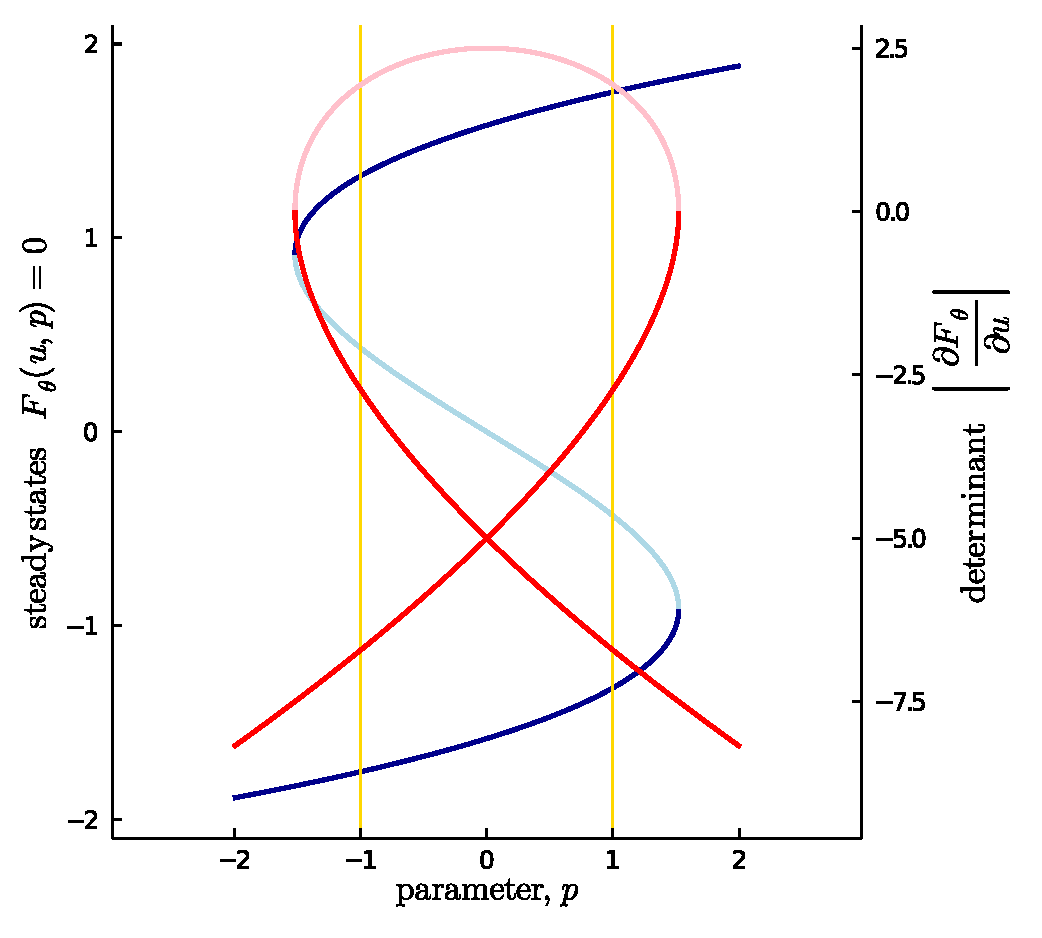
\includegraphics[width=11cm]{saddle-node}
\caption{Saddle-node model $\rates(z) = p + \theta_{1}u+\theta_{2}u^3$ with set $\theta=(2,-1)$ and targets $\targets=\{-1/2,1/2\}$. Lighter shades indicate the determinant crossing zero for unstable solutions}
\label{fig:saddle-node}
\end{figure}
\begin{figure}[H]
\centering{}
\captionsetup{justification=centering}
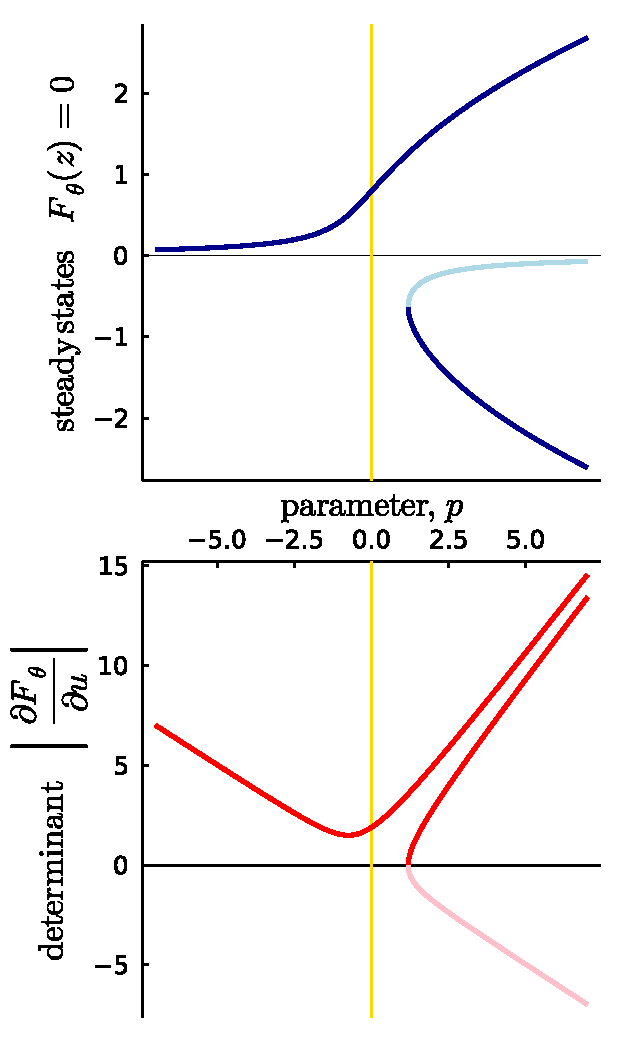
\includegraphics[width=11cm]{pitchfork}
\caption{Pitchfork model $\rates(z) = \theta_{1} + p u+\theta_{2}u^3$ with set $\theta=(-1/10,-1)$ and target $\targets=\{0\}$. Lighter shades indicate the determinant crossing zero for unstable solutions}
\label{fig:pitchfork}
\end{figure}

\subsection{Bifurcation Curves as Tangent Fields}
Obtaining a bifurcation curve involves solving for the steady states of \eqref{eq:model} along bifurcation parameter $p$. This is equivalent to finding the intersection between $N$ surfaces where each surface is given by a component of the rate function $\rates$. Each surface is embedded in $\Reals^{N+1}$ since the bifurcation parameter $p$ is an additional unknown variable. Thus the co-dimension one bifurcation curve is an $N+1$ dimensional implicit space curve defined by the $N$ equations
\begin{align}
    \rates(z) = 0
\end{align}

\begin{figure}[H]
\centering{}
\captionsetup{justification=centering}
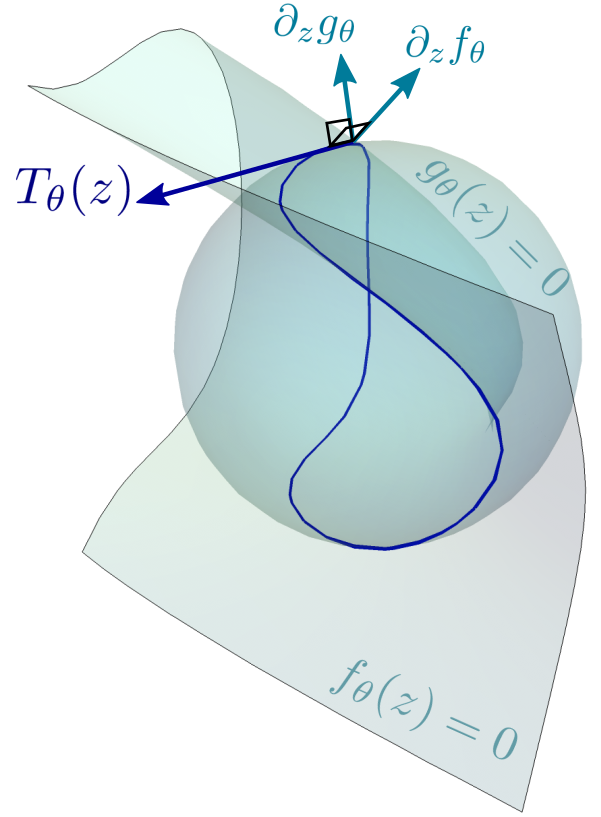
\includegraphics[width=6cm]{implicit-surfaces}
\caption{Two implicit surfaces $f_{\theta}(z)=0$ and $g_{\theta}(z)=0$ in $\mathbb{R}^3$ intersecting to form a\\ space curve which is tangent to field $\tangent(z)$ and perpendicular to gradients $\partial_{z}f_{\theta}$ and $\partial_{z}g_{\theta}$}
\label{fig:implicit-surfaces}
\end{figure}

An expression for the field $\tangent(z)$ tangent to the bifurcation curve would allow us to take derivatives and integrals along it. Fortunately the tangent field can be constructed by ensuring it is perpendicular to the gradient $\partial_z$ of each component of $\rates$ as illustrated by an example two component system in Figure \ref{fig:implicit-surfaces}. The tangent field $\tangent(z)$ can be constructed perpendicular to all gradient vectors using the properties of the determinant \cite{Goldman2005CurvatureSurfaces}
\begin{align}
    \tangent(z):=
    \left|\begin{matrix}
        \hat{z} \\
        \,\partial_{z}\rates\,
    \end{matrix}\right|
    \qquad\mathrm{where}\quad
    \hat{z}:=(\hat{u},\hat{p})\quad
	\tangent : \Reals^{N+1}\rightarrow\Reals^{N+1}
	\label{eq:tangent-field}
\end{align}
where $\hat{z}$ is a collection of unit basis vectors in the $\Reals^{N+1}$ space and $\partial_{z}\rates$ is an $N\times(N+1)$ augmented Jacobian matrix of partial derivatives including $\partial_p \rates$ in the last column. This construction ensures that the dot product of this field any gradient of a component of $\rates$
\begin{align}
    \tangent(z)\cdot\partial_z f_{\theta} =
    \left|\begin{matrix}
        \partial_z f_{\theta} \\
        \,\partial_{z}\rates\,
    \end{matrix}\right|
    \quad =0 \quad\forall f_{\theta}\in \rates
\end{align}
since the determinant of any matrix with two identical rows or columns is zero. Note that the tangent field $\tangent(z)$ is actually defined for all values of $z$ where adjacent field lines trace out other solutions where rates $\rates(z)\neq0$.

\begin{figure}[H]
\centering{}
\captionsetup{justification=centering}
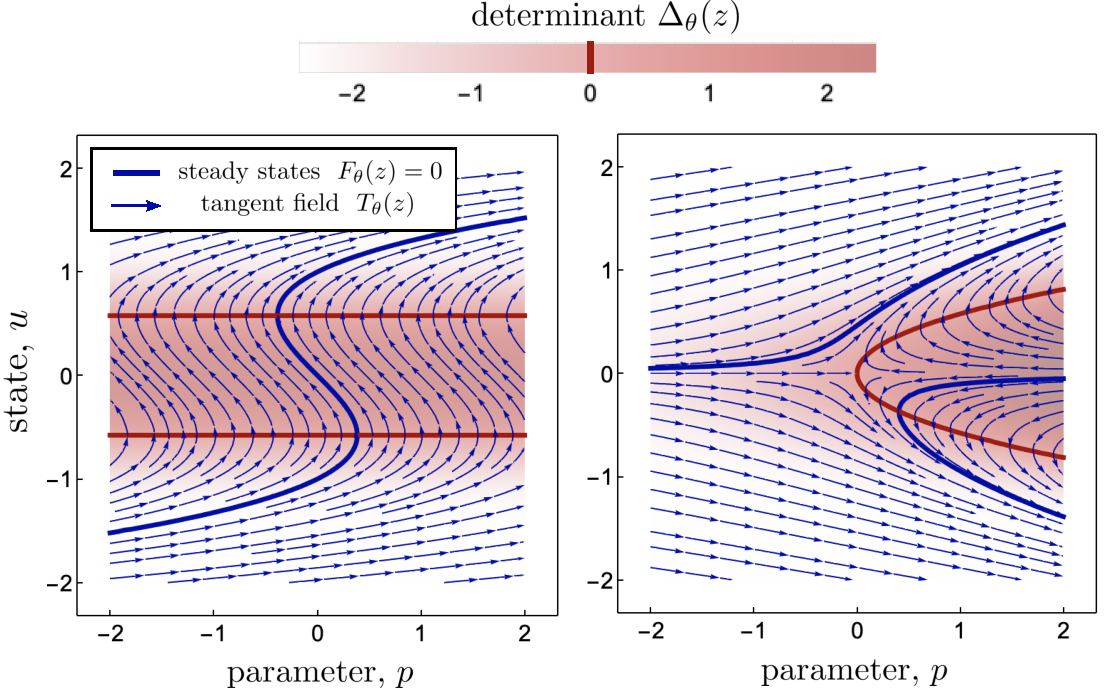
\includegraphics[width=14cm]{determinant-curvature}
\caption{Left/Right : Determinant $\Det(z)$ and tangent field $\tangent(z)$ for the saddle-node/pitchfork models for some set values of $\theta$ revealing that $\Det(z)=0$ defines bifurcations}
\label{fig:determinant-curvature}
\end{figure}

Figure \ref{fig:determinant-curvature} shows how the bifurcation curve defined by $\rates(z)=0$ picks out one of many traces in tangent field $\tangent(z)$ for the saddle and pitchfork. The tangent field $\tangent(z)$ can always be analytically evaluated by taking the determinant in \eqref{eq:tangent-field}. We will proceed with calculations on $\tangent(z)$ in the whole space $z$ and pick out a single trace by solving $\rates(z)=0$ later. For our two models
\begin{align}
    \underset{\mathrm{saddle-node\,\,model}}{
    \tangent(z)=\hat{u}-(\,3\theta_2 u^2+\theta_1\,)\,\hat{p}}
    \qquad\qquad
    \underset{\mathrm{pitchfork\,\,model}}{
    \tangent(z)=u\hat{u}-(\,3\theta_2 u^2+p\,)\,\hat{p}}
    \label{eq:tangent-field-examples}
\end{align}

\subsection{Evaluating Curvature of the Determinant}
Bifurcation points are defined as values of $z$ along the bifurcation curve where eigenvalues $\lambda$ of the Jacobian $\partial_u \rates(z)$ cross either the real or imaginary axis in the complex plane. Restricting our case to $\lambda\in\Reals$ for now, it would be sufficient to look for values of $z$ where one of the eigenvalues $\lambda$ crosses zero. Therefore the determinant of the Jacobian
\begin{align}
    \Det(z) := \big|\,\partial_u \rates\,\big|
\end{align}
crossing zero can be used as a readout of whether a bifurcation has occurred. Figure \ref{fig:determinant-curvature} reveals this is indeed also true for any value $z$ --- not just along $\rates(z)=0$ --- for the saddle-node and pitchfork. The tangent field $\tangent(z)$ only folds when $\Det(z)=0$. Plotting the value of the determinant along $\rates(z)=0$ from Figure \ref{fig:determinant-curvature} would give rise to Figures \ref{fig:saddle-node} and \ref{fig:pitchfork}.

Consequently the curvature of the determinant $\partial_{\tangent}^2\Det$ along the tangent field $\tangent(z)$ in the vicinity of bifurcations tends to increase. Fortunately this curvature can always be obtained in closed analytical form. The second directional derivative with respect to tangent field $\tangent(z)$
\begin{align}
    \partial_{\tangent}^2\Det &:=
    \bigg(
        \partial_z\left(
            \partial_z\Det \cdot \hat{\tangent}
        \right)
    \bigg)\cdot \hat{\tangent}\quad
    \mathrm{where} \quad \hat{\tangent}:=\frac{\tangent}{|\tangent|}\\
    &=
    \hat{\tangent}\cdot\partial_z^2\Det\cdot\hat{\tangent}
    \quad+\quad
    \partial_z\Det\cdot\partial_z\hat{\tangent}\cdot\hat{\tangent}
\end{align}
The first term in the expression above is the usual result involving the Hessian matrix $\partial_z^2\Det$ when taking second order directional derivatives. The second term involving the gradient $\partial_z\Det$ appears because $\hat{\tangent}(z)$ is a function of $z$ giving rise to a non-zero Jacobian matrix $\partial_z \hat{\tangent}$. Using expressions for tangent fields \eqref{eq:tangent-field-examples} and determinants for the saddle-node and pitchfork models the determinant curvatures respectively become
\begin{align}
    \underset{\mathrm{saddle-node\,\,model}}{
    \partial_{\tangent}^2\Det =
    -\frac{6 \theta_2 \left(\theta _1^2-9 \theta _2^2 u^4+1\right)}
    {\left(\left(\theta _1+3 \theta _2 u^2\right){}^2+1\right){}^2}}
    \qquad
    \underset{\mathrm{pitchfork\,\,model}}{
    \partial_{\tangent}^2\Det =
    -\frac{2 u^2 \left(p+3 \theta _2 u^2\right) \left(9 \theta _2 \left(p+\theta _2 u^2\right)+1\right)}{
    ( \left(p+3 \theta _2 u^2\right)^2+u^2 )^2
    }}
\end{align}
\subsection{Semi-supervised Cost Function}

This curvature of the determinant $\partial_{\tangent}^2\Det$ can be extremised to encourage bifurcations. We can treat this curvature as an unsupervised correction of magnitude $\lambda$ to a supervised likelihood $L_{\theta}(z|\targets)$. For a particular bifurcation curve defined by $\rates(z)=0$ we can express the cost function as the negative log-likelihood
\begin{align}
    \loss(\theta|\targets) := -\log\left(\int_{\rates(z)=0}\!
    L_{\theta}(z|\targets) + \lambda\,K_{\theta}(z)^2\,
    \,\mathrm{d}z\right)\\
    L_{\theta}(z|\targets) := \mathbb{e}^{-|\targets-p|^2/\varepsilon-\Det(z)^2}\qquad
     K_{\theta}(z):=\frac{\partial^2\Det}{\partial\tangent^2}
\end{align}
where we have chosen a Gaussian likelihood to bias optimisation of points in $z$ where the determinant $\Det(z)$ is close to zero towards targets $\targets$. Figure \ref{fig:likelihood} shows how the likelihood $L_{\theta}(z|\targets)$ is sharply peaked around the bifurcation points $\predictions(\theta)$ and is maximal when they match the targets. The parameter $\varepsilon$ controls the desired precision of the likelihood function and $\lambda$ controls the strength of the unsupervised bias.

\begin{figure}[H]
\centering{}
\captionsetup{justification=centering}
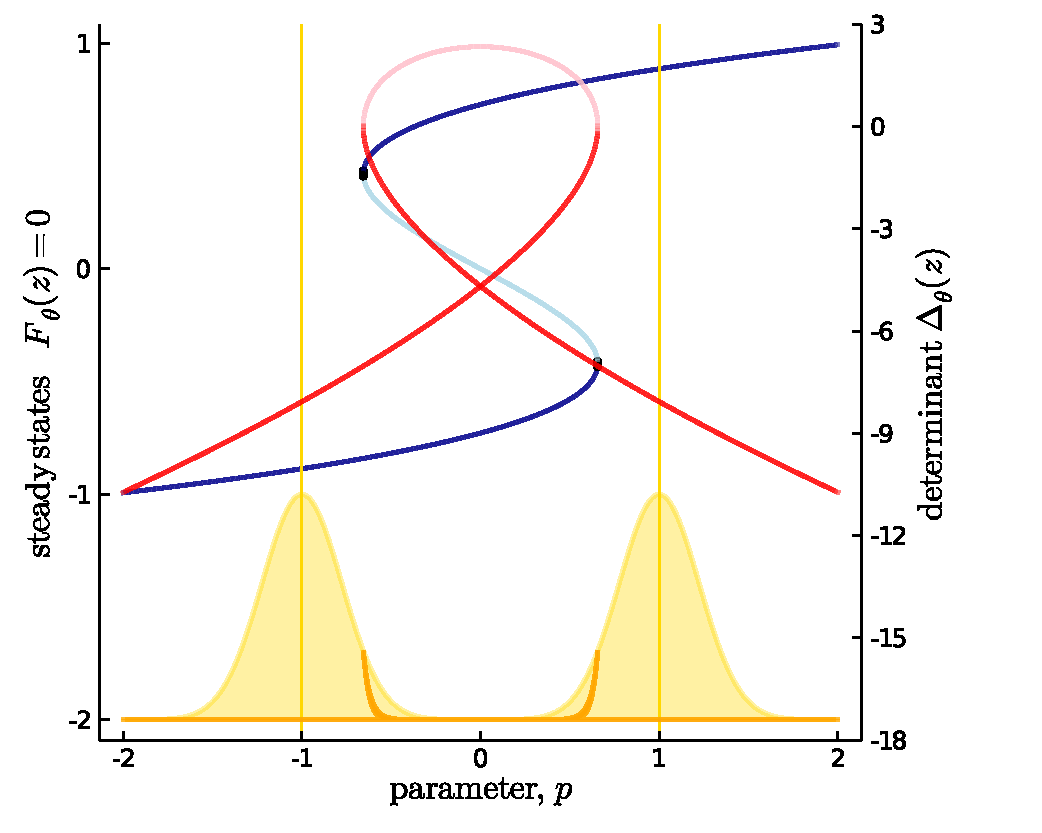
\includegraphics[width=7cm]{likelihood-1.pdf}
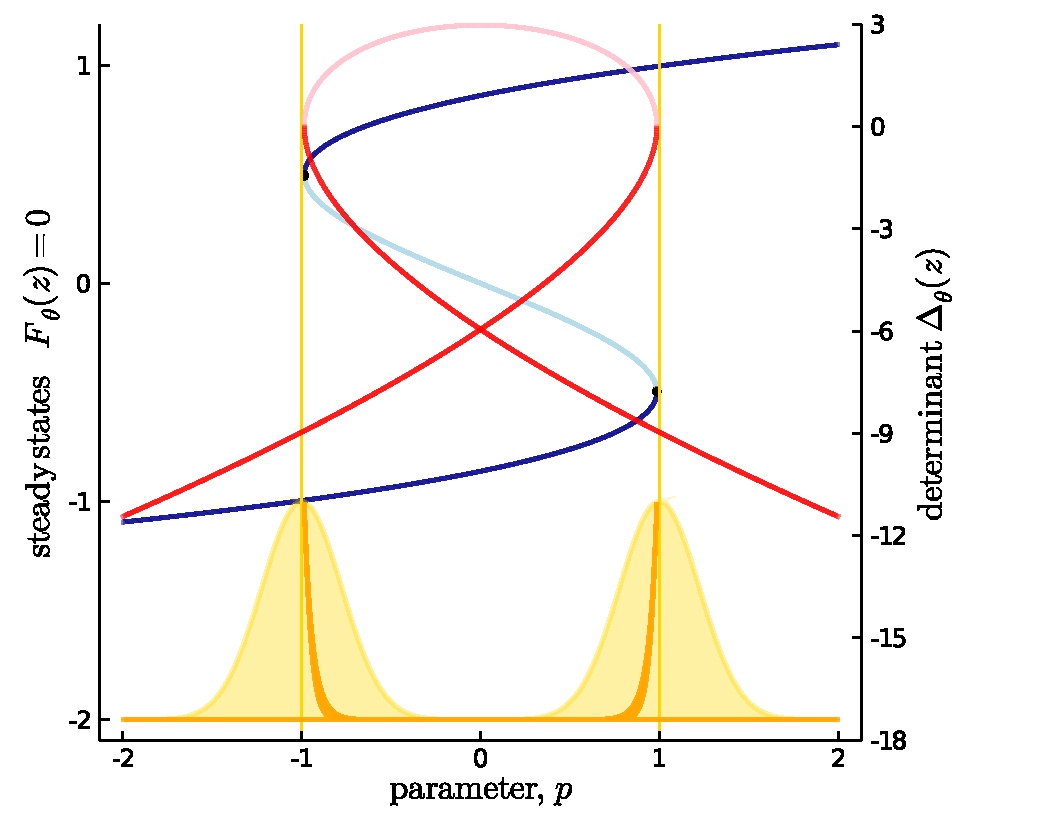
\includegraphics[width=7cm]{likelihood-2.pdf}
\caption{Likelihood $L_{\theta}(z|\targets)$ shown in dark gold is sharply peaked around the bifurcation points $\predictions(\theta)$ and is maximal when they match the targets (Right). The light gold envelope shows the maxima of the likelihood as the points $\predictions(\theta)$ sweep across different values of $p$}
\label{fig:likelihood}
\end{figure}
Applying the gradient operator with respect to $\theta$ to the cost function, we find that not only the integrand but also the integration region needs to be differentiated. This requires the general Leibniz rule \cite{Flanders1973DifferentiationSign} which yields
\begin{align}
\frac{\partial\loss(\theta|\targets)}{\partial\theta}=
-\frac{
\int_{F=0}
  \mathrm{div}\!
\left(\frac{\partial z}{\partial\theta}
  \left(L+\lambda K^2\right)
\right)
+\frac{\partial L}{\partial\theta}+
2\lambda K\frac{\partial K}{\partial\theta}
\,\,\mathrm{d}z
}{
\int_{F=0}
\left(
  L+\lambda K^2
\right)\,\mathrm{d}z
}\label{eq:gradient}
\end{align}
where $\frac{\partial z}{\partial\theta}$ is the velocity field of the integration region due to changes in $\theta$. Fortunately the velocity field of implicitly defined regions can be solved for analytically \cite{Jos2011OnSurface}. This is done by taking the total derivative of the implicit equation
\begin{align}
    \frac{d\rates(z)}{d\theta}=\frac{\partial F}{\partial\theta}+
    \frac{\partial F}{\partial z}\frac{\partial z}{\partial\theta}
\end{align}
We can rearrange for $\frac{\partial z}{\partial\theta}$ using the Moore-Penrose inverse of the augmented Jacobian matrix $\frac{\partial F}{\partial z}$ which appeared in equation \eqref{eq:tangent-field}. Since the surface is defined by $\rates(z)=0$ we arrive at
\begin{align}
    \frac{\partial z}{\partial\theta} = - \frac{\partial F}{\partial z}^\top
    \left(\,
        \frac{\partial F}{\partial z}\,\frac{\partial F}{\partial z}^\top
    \right)^{-1}
    \frac{\partial F}{\partial\theta}
\end{align}
which for our two minimal models yield
\begin{align}
    \underset{\mathrm{saddle-node\,\,model}}{
    \frac{\partial z}{\partial\theta} =
        \frac{ \hat{p}+\hat{u}\,(\,\theta_1+3\theta_2 u^2\,) }{1+(\,\theta_1+3\theta_2 u^2\,)^2}
        \left( u\,\hat{\theta}_1 + u^3\,\hat{\theta}_2 \right)}
    \qquad
    \underset{\mathrm{pitchfork\,\,model}}{
    \frac{\partial z}{\partial\theta} =
        \frac{ p\,\hat{u} + u\,(\,\hat{p}+3\theta_2u\,\hat{u}\,) }{(\,p+3\theta_2 u^2\,)^2 + u^2 }
        \left( \hat{\theta}_1 + u^3\,\hat{\theta}_2 \right)}
    \label{eq:velocity-field-examples}
\end{align}
Thus the integrands in the gradient \eqref{eq:gradient} are completely analytic, leaving only region $\rates(z)=0$ to be evaluated numerically. Since these analytic forms can be pre-calculated, calculating the gradients shares the same computational complexity as calculating the steady states. 
% \subsection{Basis Functions and Unsupervided Bias}
% \subsection{Pseudo-arclength Continuation}

\subsection{Optimisation Loop}
Here provide a high-level view of Algorithm \ref{alg:optimisation-loop}. We use \texttt{BifurcationKit.jl} \cite{Veltz2019PseudoArcLengthContinuation.jl} to calculate bifurcation diagrams, which requires the rate function $\rates$, its Jacobian $J_\theta$, and an initial guess $u_0$ at an initial parameter $p_0$. Let this algorithm be called by function $\mathrm{getSteadyStates}$ and return the steady states that form the integration region $\Omega$ and a new guess $u_0$ that is the true steady state at $p_0$.

The algorithm also takes hyperparameters $\beta$ which will contain arclength step sizes, eigenvalue and Newton solver options and unsupervised correction factor $\lambda$. The adaptive hyperparameter update is done by $\mathrm{updateHyperparameters}$ and should depend on the current solutions $\Omega$ and the targets $\targets$. The step sizes and solver options should adapt to the expected space of the solutions $\Omega$ so that the waiting time between iterations is minimised. The unsupervised correction factor $\lambda$ should be large when there are no predicted bifurcations and decrease as the number of predicted bifurcations approaches the number of targets.

The evaluation of the cost gradient \eqref{eq:gradient} is done by $\mathrm{costGradient}$ using \texttt{Zygote.jl} \cite{Innes2018DontPrograms} and requires the following analytical forms: the determinant of the Jacobian $\Det$, its curvature $K_{\theta}$ and the integration region velocity $\frac{\partial z}{\partial\theta}$. It also requires the integration region $\Omega$ and the locations of targets $\targets$. This gradient is used by $\mathrm{updateParameters}$, which can be any gradient-based optimiser such as ADAM or Momentum gradient decent, to update the parameters $\theta$.
\\\\
\begin{algorithm*}[H]
\label{alg:optimisation-loop}
\SetAlgoLined
\textbf{Inputs} Function $F_{\theta}:\mathbb{R}^{N+1}\rightarrow\mathbb{R}^{N}$ for $u\in\mathbb{R}^N$ and $p\in\mathbb{R}$\\ target bifurcations $\mathcal{D}=\{p:p\in[p_{\min},p_{\max}]\}$ and convergence tolerance $\varepsilon$\\
\textbf{Output} Optimised $\theta\in\mathbb{R}^M$ that satisfy targets $\targets$\\
$J_{\theta}\leftarrow\partial F/\partial u$\qquad\,
$\Delta_{\theta}\leftarrow|\mathrm{det}\,J_{\theta}|$\qquad$K_{\theta}\leftarrow\partial^2\Delta_{\theta}/\partial\tangent^2$\\
$\frac{\partial z}{\partial\theta}\leftarrow- \frac{\partial F}{\partial z}^\top
    \left(\,
        \frac{\partial F}{\partial z}\,\frac{\partial F}{\partial z}^\top
    \right)^{-1}
    \frac{\partial F}{\partial\theta}$\\
$u_0\leftarrow\mathrm{rand}\in\mathbb{R}^{N}$\quad\,$\theta\leftarrow\mathrm{rand}\in\mathbb{R}^{M}$\\
$\beta\leftarrow\mathrm{getHyperparameters}(\targets)$\\
\While{$\mathrm{tolerance}(\beta)>\varepsilon$}{
  $\Omega,u_0\leftarrow\mathrm{getSteadyStates}(F_{\theta},J_{\theta},u_0,\beta)$\\
  $\beta\leftarrow\mathrm{updateHyperparameters}(\beta,\Omega,\targets)$\\
  $\partial L\leftarrow\mathrm{costGradient}(\Delta_{\theta},K_{\theta},\frac{\partial z}{\partial\theta},\Omega,\targets)$\\
  $\theta\leftarrow\mathrm{updateParameters}(\theta,\partial L,\beta)$
}
\caption{Bifurcation Optimisation Loop}
\end{algorithm*}

\section{Results}

\subsection{Model Synthesis}


\subsection{Model Selection}




\section{Conclusions and Extensions}
\label{sec:conclusions}

\begin{itemize}
    \item cell cycle / hopf
    \item application to structure $\rightarrow$ function (Luca)
    \item pattern formation in pdes
\end{itemize}

\bibliography{refs}
\bibliographystyle{ieeetr}
\end{document}
